Cette partie de l'algorithme a pour but de redéfinir les classes des pixels proches des frontières entre 2 régions afin de supprimer les nœuds isolés (ceux qui ont une classe différentes de ceux qui l'entourent), et ainsi de diminuer les erreurs. Cette partie s'organise en trois étapes : identification des nœuds appartenant à la frontière, leur lissage via l'application d'un filtre linéaire et la réaffectation des classes. Ces étapes sont effectuées sur chaque niveau du quadtree.

\subsection{Identification de la frontière}
	Nous allons tout d'abord chercher à identifier les nœuds situés sur la frontière entre deux régions. Pour cela nous allons travailler sur le niveau $m'$ du quadtree, sur lequel la classification a été effectuée, et sur l'image correspondante.\\

	Un pixel appartient à la frontière $B(k)$ si un des ces huit voisins possède une classe différente de celle du pixel. Ainsi :

	\[ q(i,j,k) \in B(k) \Leftrightarrow c[q(i,j,k)] \ne c[q(i',j',k)] \]
	\[ (i',j') \in N_8(i,j) \]

	En appliquant ceci à chaque pixel de l'image nous avons déterminé lesquels appartenaient à $B(k)$. Prenons par exemple une frontière en ligne droite comme dans la figure \ref{fig:bordure}.

	\begin{figure}[H]
		\centering
		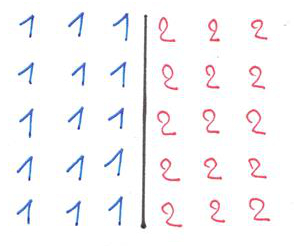
\includegraphics[scale=0.75]{images/bordure.jpg}
		\caption{Frontière en ligne droite entre 2 classes}
		\label{fig:bordure}
	\end{figure}

	$B(k)$ sera alors défini selon la figure \ref{fig:bordure2}.\\
	\begin{figure}[H]
		\centering
		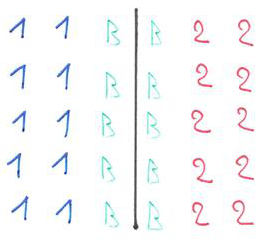
\includegraphics[scale=0.75]{images/bordure-2.jpg}
		\caption{Frontière en ligne droite entre 2 classes avec apparition de la première bordure}
		\label{fig:bordure2}
	\end{figure}

	Nous allons maintenant chercher à déterminer $B_1(k)$. L'union de $B(k)$ et de $B_1(k)$ nous donnera les pixels appartenant aux frontières.\\

	Un pixel appartient à $B_1(k)$ si un des ses huit voisins appartient à $B(k)$. Ainsi la frontière que nous avions définie précédemment \enquote{s'épaissit}. On obtient :

	\[ q(i,j,k) \in B_1(k) \Leftrightarrow q(i',j',k) \in B(k) \]
	\[ (i',j') \in N_8(i,j) \]

	et \[ B_c(k) = B(k) \cup B_1(k) \]

	Ainsi pour l'exemple précédent nous obtenons la figure \ref{fig:bordure3}. Nous allons maintenant travailler sur $B_c(k)$, que nous considérons comme notre frontière.

	\begin{figure}[H]
		\centering
		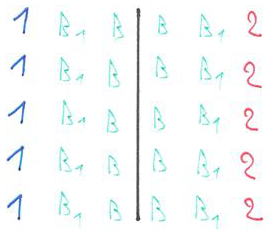
\includegraphics[scale=0.75]{images/bordure-3.jpg}
		\caption{Frontière en ligne droite entre 2 classes avec union des bordures}
		\label{fig:bordure3}
	\end{figure}

\subsection{Lissage}
	Maintenant que nous connaissons les pixels appartenant à la frontière $B_c(k)$, nous allons les lisser grâce à une filtre linéaire. Nous allons maintenant définir le filtre linéaire utilisé.
	On note $\hat{\mu}_1$ et $\hat{\mu}_2$ les moyennes des deux classes que la frontière sépare et $\hat{\mu}(i,j,k)$ la moyenne de la classe associée au pixel $(i,j,k)$.\\

	Soit $B_c'(k)$ l'ensemble des pixels n'appartenant pas à la frontière.On définit :

	\[ \hat{\sigma}_k^2 = \frac{\sum\limits_{(i,j) \in B_c'(k)}[q(i,j,k)-\hat{\mu}(i,j,k)]^2}{N(B_c'(k))} \]

	$N(A)$ correspondant au nombre de points à l'intérieur de la région $A$.

	Soit :
	\[ \hat{\rho}_k = \frac{\hat{\mu}_1 - \hat{\mu}_2}{\hat{\sigma}_k^2} \]

	Notre filtre linéaire est alors défini par :

	\[ h(\rho) = \left\lbrace\begin{array}{cc}
		\lambda(\rho) & \mbox{si } (i,j) = (0,0), \\
		\frac{1 - \lambda(\rho)}{8} & \mbox{sinon}\\
	\end{array}\right.
	\]

	$\lambda(\rho)$ étant une fonction linéaire par partie de $\rho$.

	On applique le filtre en effectuant une convolution :
	\[ B_2(k) = h(i,j,\hat{\rho}_k) * B_c(k) \]

\subsection{Réaffectation des classes}
	L'application du filtre nous a permis de lisser les pixels appartenant à la frontière. Nous allons maintenant réaffecter leurs classes à ces pixels en leur attribuant la classe dont la moyenne est la plus proche.

\subsection{Répétition aux autre niveaux}
	Les trois étapes précédentes sont répétées aux niveaux inférieurs du quadtree. On doit tout d'abord affecter les classes aux pixels en affectant aux fils la même classe que leur père. On applique ensuite à ce niveau l'identification de la frontière, le lissage et l'affection des classes. On répète l'opération au niveau inférieur et ainsi de suite jusqu'au niveau $k=0$, correspondant aux données initiales.